\chapter{System Design}

\section{Review of Workshop No. 1 Findings}
\subsection{Summary of Systems Analysis}

In Workshop 1, we conducted a comprehensive systems analysis of the CIBMTR Kaggle competition focused on equity in post-HCT survival predictions. Our analysis revealed the complex nature of the medical system surrounding hematopoietic cell transplantation procedures, characterized by multiple interconnected clinical, genetic, and demographic factors that influence patient outcomes.

Key findings from our analysis include:

\begin{itemize}
    \item \textbf{System Components:} The system comprises diverse data sources including disease characteristics, transplant-specific inputs, demographic factors, and temporal variables, all contributing to survival predictions.
    
    \item \textbf{High Complexity:} Post-HCT survival prediction involves nonlinear interactions between variables, forming a high-dimensional system where small parameter changes can lead to significant outcome differences.
    
    \item \textbf{Sensitivity Analysis:} We identified critical sensitivity parameters including patient age, disease risk indices, genetic compatibility scores, and comorbidities, where minor variations can dramatically alter survival predictions.
    
    \item \textbf{Chaos Theory:} Medical outcomes following HCT exhibit characteristics of chaos theory and inherent randomness, where small inaccuracies in measurements can lead to unpredictable outcomes.
    
    \item \textbf{Equity Considerations:} The stratified C-index metric ensures model performance is consistent across ethnic subgroups, highlighting the need for fairness-aware modeling approaches.
\end{itemize}

Our analysis emphasized the importance of addressing both the technical challenges of accurate prediction and the ethical imperatives of ensuring equitable performance across diverse patient populations.

\subsection{Critical Constraints}

Our analysis from Workshop 1 identified several critical constraints that must be addressed in our system design:

\begin{itemize}
    \item \textbf{Data Limitations:} The competition restricts participants to use only the provided CIBMTR datasets, without external data sources. This constraint limits our ability to supplement missing information or incorporate additional variables that might improve predictive performance.
    
    \item \textbf{Fairness Requirements:} The system must meet stringent equity criteria, ensuring similar performance across different demographic groups as measured by the stratified C-index. This requires explicit fairness considerations throughout the modeling pipeline.
    
    \item \textbf{Clinical Validity:} Predictions must maintain medical relevance and interpretability for real-world application. Solutions that achieve high mathematical accuracy without clinical meaningfulness would fail to meet the competition's underlying healthcare objectives.
    
    \item \textbf{Missing Data Patterns:} The dataset contains significant missing values with patterns that may vary systematically across demographic groups. The system must handle missing data in ways that don't amplify existing disparities.
    
    \item \textbf{Computational Feasibility:} While complex modeling approaches are needed to capture the system's nonlinear nature, solutions must remain computationally feasible for practical implementation and evaluation within the competition framework.
    
    \item \textbf{Temporal Validity:} Medical practices evolve over time, and models must account for potential shifts in treatment protocols and outcomes across the time span represented in the dataset.
\end{itemize}

These constraints directly inform our architectural decisions and implementation strategies, creating boundaries within which we must develop our solution.

\section{System Requirements}

\subsection{Measurable Design Requirements}

\begin{itemize}
    \item \textbf{Accuracy:} Production of results with the highest possible quality, enabling the fulfillment of user-centered needs.
    
    \item \textbf{Resilience:} Ability to maintain acceptable performance despite variations in the quantity or quality of input variables established for the system. This allows the system to properly handle generated entropy.
    
    \item \textbf{Efficiency:} Reduction in the amount of time and system resources without losing the established homeostasis in the system.
    
    \item \textbf{Scalability:} Simplicity when increasing the amount of data entered into the system.
\end{itemize}

\subsection{User-Centric Needs}

\begin{itemize}
    \item \textbf{Accuracy in post-HCT survival prediction}
    
    \item \textbf{Equity:} The model should not discriminate based on demographic or socioeconomic characteristics.
    
    \item \textbf{System resilience:} To handle missing data, outliers, and biological variability.
\end{itemize}

\begin{figure}[H]
    \centering
    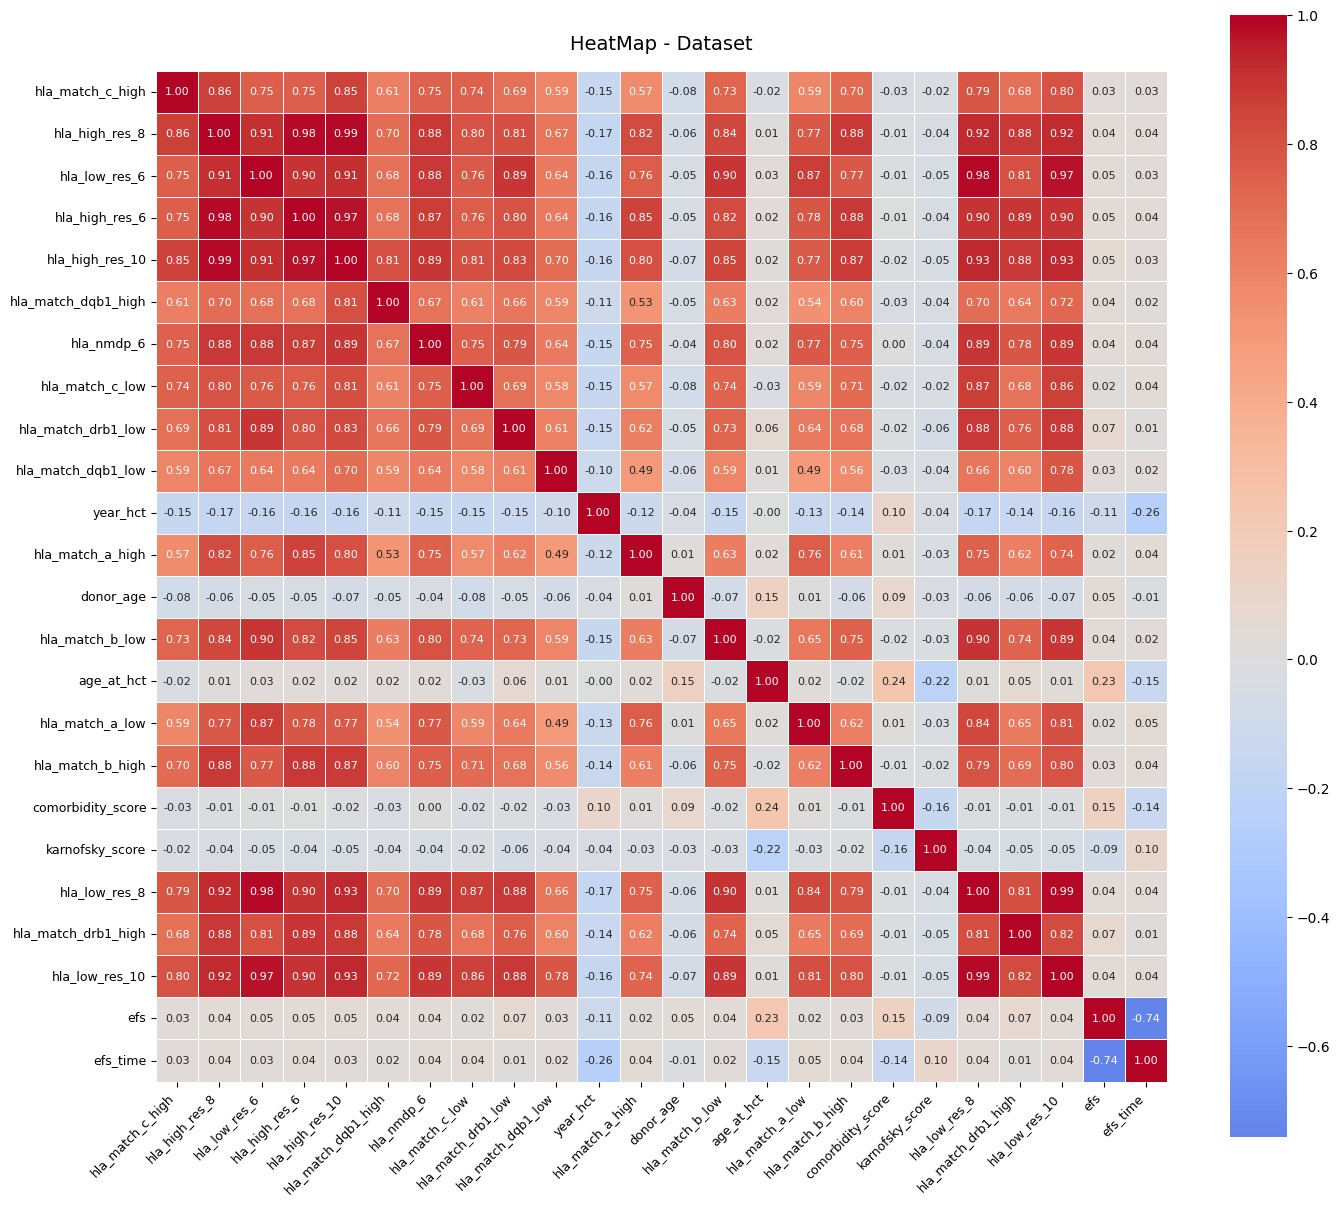
\includegraphics[width=1\textwidth]{figures/DatasetHeatmap.jpg}
    \caption{Heatmap visualization showing correlations between numerical variables in the dataset. This visualization facilitates understanding of the system's numerical input data to identify potential redundancies. By revealing which variables are highly correlated with each other, the heatmap provides insight into variable relationships that may influence system performance. This understanding allows us to prioritize relationships that contribute most effectively to the established system requirements, particularly with respect to equity considerations across demographic groups.}
    \label{fig:dataset_heatmap}
\end{figure}

\subsection{Evaluation Metric and Fairness Assessment}

The stratified C-index serves as the primary evaluation metric for this system, designed specifically to ensure equity across demographic groups. This metric is central to the competition objectives and directly informs our architectural decisions.

\begin{figure}[H]
    \centering
    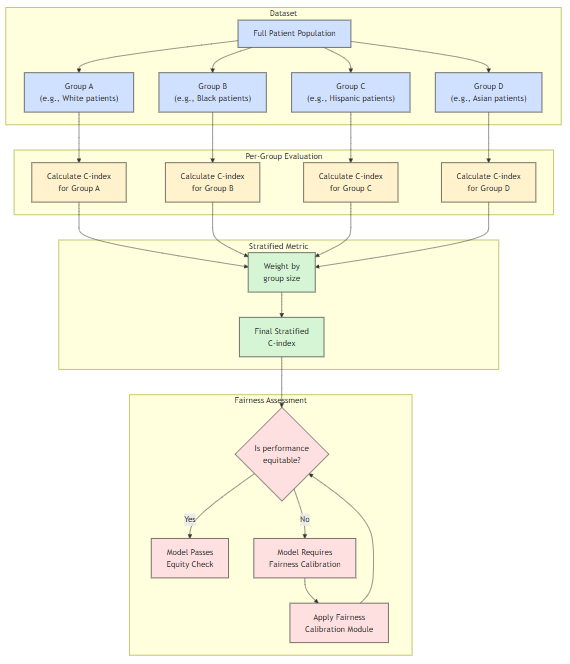
\includegraphics[width=0.95\textwidth]{figures/StratifiedCindexDiagram.png}
    \caption{Workflow for calculating the stratified C-index and performing fairness assessment. The process begins with stratification of the patient population by demographic groups, followed by separate C-index calculation within each group. These group-specific metrics are then weighted according to group size to produce the final stratified C-index. The fairness assessment loop ensures models deliver equitable performance across all patient populations, triggering fairness calibration when necessary.}
    \label{fig:cindex_fairness_diagram}
\end{figure}

This evaluation approach addresses a critical challenge in healthcare prediction: models may perform well on average while performing poorly for specific demographic groups. By requiring consistent performance across all patient populations, the stratified C-index incentivizes fair prediction systems that do not disadvantage underrepresented groups. Our architecture explicitly addresses this requirement through dedicated modules for equity analysis and fairness calibration.

\section{High-Level Architecture}

\subsection{Architectural Overview}

The system architecture is founded on a modular and sequential pipeline that aims to optimize clinical accuracy and equity, responding to the complexity and high sensitivity identified in Workshop No. 1.

The architecture of the system is organized into modules representing the main stages, from the ingestion of raw data (clinical, genetic, and demographic data) to the generation of predictions and equity metrics for clinical decision support.

\begin{figure}[H]
    \centering
    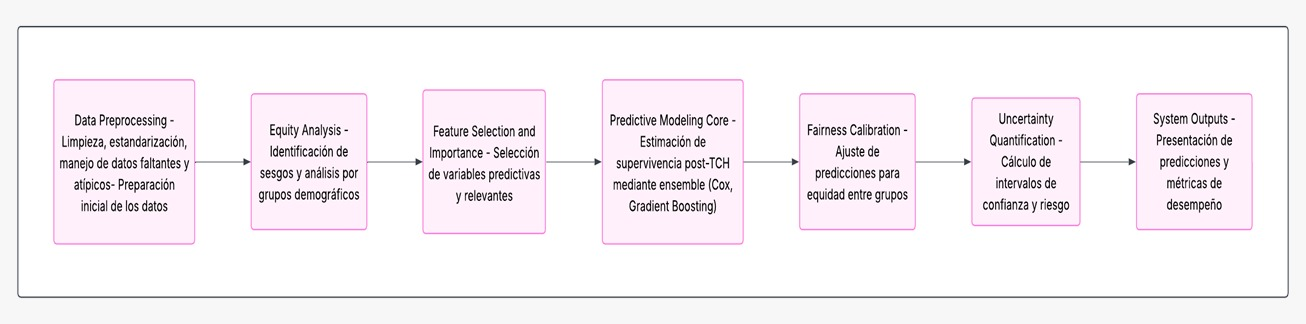
\includegraphics[width=1\textwidth]{figures/SystemDesignArchitecture.jpg}
    \caption{High-level architecture showing the seven core modules and data flow for the post-HCT survival prediction system.}
    \label{fig:system_architecture_design}
\end{figure}

\subsection{Modules and Responsibilities}

The architecture consists of seven interconnected modules, each with a specific responsibility:

\subsubsection{1. Data Preprocessing Module}

\begin{table}[H]
\centering
\begin{tabular}{|p{5cm}|p{9cm}|}
\hline
\textbf{Internal Component} & \textbf{Specific Operations} \\
\hline
Ingestion and Validation & Verifies the integrity and format of raw CIBMTR data. \\
\hline
Equity-Aware Imputation & Handles missing and atypical data. Uses methods that consider demographic variations. \\
\hline
Standardization and Normalization & Scales and transforms continuous variables (e.g., Age, laboratory values) for ML models. \\
\hline
Basic Feature Engineering & Creation of interaction features and logarithmic transformation for skewed variables. \\
\hline
\end{tabular}
\caption{Data Preprocessing Module Components and Operations}
\label{tab:preprocessing_module}
\end{table}

\subsubsection{2. Equity Analysis Module}

\begin{table}[H]
\centering
\begin{tabular}{|p{5cm}|p{9cm}|}
\hline
\textbf{Internal Component} & \textbf{Specific Operations} \\
\hline
Stratified Analysis & Performs comprehensive examination of data in demographic subgroups (e.g., Race/Ethnicity) to identify disparities in baseline outcome rates. \\
\hline
Bias Detection Algorithms & Applies algorithms to measure bias in the quality or availability of input features. \\
\hline
Balancing Techniques & Uses fairness-aware preprocessing techniques such as reweighting to improve balanced representation. \\
\hline
\end{tabular}
\caption{Equity Analysis Module Components and Operations}
\label{tab:equity_module}
\end{table}

\subsubsection{3. Feature Selection and Importance Module}

\begin{table}[H]
\centering
\begin{tabular}{|p{5cm}|p{9cm}|}
\hline
\textbf{Internal Component} & \textbf{Specific Operations} \\
\hline
Clinical Domain Integration & Prioritizes sensitive variables identified (Age, Disease Risk Index, Genetic Compatibility). \\
\hline
ML/Statistical Rankings & Ranks feature importance using methods such as Recursive Feature Elimination or statistical significance. \\
\hline
Equitable Availability Verification & Ensures that critical predictive features are consistently available across all populations. \\
\hline
\end{tabular}
\caption{Feature Selection and Importance Module Components and Operations}
\label{tab:feature_module}
\end{table}

\subsubsection{4. Predictive Modeling Core}

\begin{table}[H]
\centering
\begin{tabular}{|p{5cm}|p{9cm}|}
\hline
\textbf{Internal Component} & \textbf{Specific Operations} \\
\hline
Proportional Hazards Models (Cox) & Base models for time-to-event survival predictions. \\
\hline
Ensemble Algorithms & Uses Gradient Boosting Machines (GBMs) and Random Forests to capture non-linear patterns. \\
\hline
Deep Learning Architectures & Implements neural models for complex non-linear relationships, when necessary. \\
\hline
Cross-Validation Strategy & Executes demographically stratified cross-validation adapted for survival data. \\
\hline
\end{tabular}
\caption{Predictive Modeling Core Components and Operations}
\label{tab:modeling_module}
\end{table}

\subsubsection{5. Fairness Calibration Module}

\begin{table}[H]
\centering
\begin{tabular}{|p{5cm}|p{9cm}|}
\hline
\textbf{Internal Component} & \textbf{Specific Operations} \\
\hline
Probability Calibration & Adjusts survival curves to maintain comparable accuracy across different patient populations. \\
\hline
Risk Threshold Optimization & Modifies risk classification thresholds (low, intermediate, high) to minimize disparity in risk assessment. \\
\hline
Disparity Impact & Quantifies the effect of adjustments to ensure minimization of prediction inequities. \\
\hline
\end{tabular}
\caption{Fairness Calibration Module Components and Operations}
\label{tab:fairness_module}
\end{table}

\subsubsection{6. Uncertainty Quantification Module}

\begin{table}[H]
\centering
\begin{tabular}{|p{5cm}|p{9cm}|}
\hline
\textbf{Internal Component} & \textbf{Specific Operations} \\
\hline
Prediction Interval Calculation & Generates confidence intervals using methods appropriate for survival analysis. \\
\hline
Risk and Reliability & Associates uncertainty bounds with risk stratification. \\
\hline
Low Reliability Identification & Flags cases where prediction is less reliable due to incomplete or atypical data. \\
\hline
\end{tabular}
\caption{Uncertainty Quantification Module Components and Operations}
\label{tab:uncertainty_module}
\end{table}

\subsubsection{7. System Outputs}

\begin{table}[H]
\centering
\begin{tabular}{|p{5cm}|p{9cm}|}
\hline
\textbf{Internal Component} & \textbf{Specific Operations} \\
\hline
Prediction Generator & Produces survival probabilities and risk stratification categories. \\
\hline
Equity Metrics Dashboard & Displays equity assessment and prediction consistency across groups. \\
\hline
Interpretation Engine (SHAP) & Generates detailed explanations for individual predictions (SHAP values, Feature Importance). \\
\hline
Quality and QA Reports & Delivers performance metrics, calibration plots, and data quality reports. \\
\hline
\end{tabular}
\caption{System Outputs Components and Operations}
\label{tab:outputs_module}
\end{table}

\subsection{Systems Engineering Principles}

The systems engineering principles applied to shape these structural decisions are:

\begin{itemize}
    \item \textbf{Modularity:} The architecture is divided into discrete modules, allowing independent development, testing, and component replacement without affecting overall system integrity.
    
    \item \textbf{Scalability:} The pipeline design supports complex methods such as ensemble modeling and stratified analysis. This ensures the system can handle both the high volume of data from CIBMTR and the computational complexity required.
    
    \item \textbf{Maintainability:} Clear documentation and separation of tasks are integrated. This separation facilitates audits and updates in response to new medical advances or equity requirements.
    
    \item \textbf{Robustness and Complexity Management:} 
    \begin{itemize}
        \item The inclusion of the Uncertainty Quantification Module and the use of ensemble models mitigate the effects of chaotic behavior and high system sensitivity (where small changes in input generate large changes in output).
        \item The Fairness Calibration Module reinforces system robustness against latent biases and ensures that the critical stratified C-Index metric is consistently met across all populations.
    \end{itemize}
\end{itemize}

\subsection{Complexity and Sensitivity Analysis}

\subsubsection{Complexity in Post-HCT Survival Modeling}

The challenge of predicting survival outcomes after hematopoietic cell transplantation (HCT) centers fundamentally on the system's inherent complexity \cite{astct_simplification}. Multiple interconnected clinical, genetic, and demographic factors influence patient survival outcomes, creating a nonlinear, high-dimensional system where minor parameter variations can produce significant outcome differences \cite{frontiers_ai_hct}.

As identified in our analysis, post-HCT survival prediction involves:

\begin{itemize}
    \item Multifactorial disease characteristics that vary by hematologic malignancy type \cite{ash_transplant_all}
    \item Complex donor-recipient genetic compatibility factors affecting engraftment \cite{mdpi_cells}
    \item Demographic variables with potential impact on healthcare access and outcomes \cite{jama_ai_medicine}
    \item Temporal aspects reflecting evolving medical practices over the dataset's time span \cite{mdpi_cancers}
\end{itemize}

Feedback mechanisms such as immune responses, graft-versus-host disease, and intervention-triggered complications further complicate prediction by introducing additional nonlinearity \cite{ash_chronic_gvhd}.

\subsubsection{Sensitivity Analysis}

Our analysis identified several parameters where small variations generate disproportionate impact on survival predictions:

\begin{itemize}
    \item \textbf{Age:} Even a single-year difference can shift risk categorization significantly for patients near clinical thresholds \cite{stmcls_clonality}
    \item \textbf{Disease risk indices:} Minor score changes can alter treatment eligibility and prognosis \cite{uptodate_hct}
    \item \textbf{HLA matching:} Subtle genetic compatibility differences substantially affect transplant rejection rates \cite{frontiers_immunology}
    \item \textbf{Comorbidities:} Presence or absence of specific conditions can dramatically alter survival projections \cite{mdpi_cancers}
\end{itemize}

\begin{figure}[H]
    \centering
    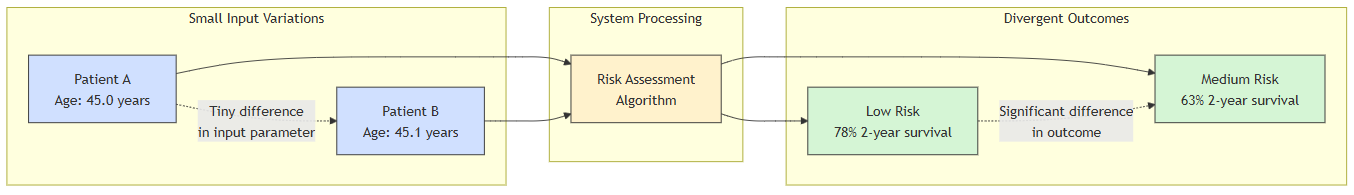
\includegraphics[width=0.95\textwidth]{figures/SensitivityDiagram.png}
    \caption{Visual representation of sensitivity in post-HCT survival prediction. This diagram illustrates how a minimal difference in patient age (just 0.1 years) can lead to significantly different risk categorization and survival probability estimates. Such high sensitivity to input parameters necessitates specialized modeling approaches that can account for these threshold effects, particularly around clinical decision boundaries.}
    \label{fig:sensitivity_diagram}
\end{figure}

\subsubsection{Chaos and Randomness in Post-HCT Survival Prediction}

Medical outcomes following allogeneic HCT exhibit characteristics of chaotic systems, where deterministic processes nonetheless produce seemingly random and unpredictable results \cite{frontiers_ai_hct}. This chaos manifests in several specific ways:

\begin{itemize}
    \item \textbf{Immune reconstitution dynamics:} Small variations in initial T-cell populations can lead to dramatically different immune recovery trajectories and corresponding survival outcomes \cite{stmcls_clonality}. Studies show that even genetically identical grafts can produce divergent immune reconstitution patterns due to sensitivity to microenvironmental conditions at transplantation.
    
    \item \textbf{Graft-versus-host disease emergence:} The development and progression of GVHD follows chaotic patterns, with similar patients on identical prophylaxis regimens experiencing vastly different disease trajectories \cite{ash_chronic_gvhd}. Minor differences in tissue damage during conditioning or subtle variations in gut microbiota can trigger significantly different inflammatory cascades.
    
    \item \textbf{Infection susceptibility:} Infection outcomes post-transplant display hallmarks of chaos theory, where minimal differences in pathogen exposure or antimicrobial timing can result in either rapid clearance or life-threatening sepsis \cite{uptodate_hct}.
    
    \item \textbf{Relapse dynamics:} For malignant conditions, disease recurrence follows complex nonlinear patterns influenced by minimal residual disease, graft-versus-leukemia effects, and immune escape mechanisms that exhibit extreme sensitivity to initial conditions \cite{mdpi_cancers}.
\end{itemize}

The ``butterfly effect'' in these systems means that conventional deterministic models struggle to capture the true range of possible outcomes. Our analysis revealed that this unpredictability is further complicated by demographic factors, as certain chaos-inducing variables (like access to prompt care for infections or monitoring for early GVHD signs) may be systematically distributed unequally across patient populations \cite{jama_ai_medicine}.

The competition's stratified C-index evaluation metric \cite{kaggle_competition} presents a particular challenge in this context, as it requires models to maintain consistent performance across demographic subgroups despite these chaotic elements. Achieving both accuracy and equity demands sophisticated approaches that can:

\begin{itemize}
    \item Quantify uncertainty ranges rather than single-point predictions
    \item Identify regions of the feature space where chaotic behavior is most likely
    \item Apply ensemble methods that capture various possible trajectory families
    \item Maintain calibration across demographic groups even when faced with inherent unpredictability
\end{itemize}

These considerations directly inform our system design, which employs multiple modeling approaches and explicit uncertainty quantification to address the fundamental chaotic nature of post-HCT outcomes while ensuring equitable performance across patient populations.

\section{Technical Stack and Implementation Sketch}

We have identified a range of widely-used and accessible tools designed to handle everything from data cleaning to results presentation, ensuring that the work can be replicated without difficulties.

\subsection{Recommended Technology Stack}

\subsubsection{Data Processing and Management Tools}

\begin{itemize}
    \item \textbf{Pandas:} Enables efficient organization and cleaning of information, such as sorting patient tables or transforming medical data \cite{geeksforgeeks_pandas}.
    
    \item \textbf{NumPy:} Facilitates rapid calculations and matrix operations, supporting all statistical processing needs \cite{dataquest_numpy}.
    
    \item \textbf{Scikit-learn:} Provides functions for data preparation, filling missing values, and splitting information for model training and validation \cite{pushkarna_preprocessing}.
\end{itemize}

\subsubsection{Survival Analysis Libraries}

\begin{itemize}
    \item \textbf{Lifelines:} This library assists in analyzing patient survival time. It includes models such as Cox Proportional Hazards and methods to calculate expected time to an event using available information \cite{lifelines_docs}.
    
    \item \textbf{Scikit-survival:} Enables the use of more advanced survival models and is compatible with other machine learning tools, making the process simpler and more integrated \cite{scikit_survival_intro}.
\end{itemize}

\subsubsection{Machine Learning Models}

\begin{itemize}
    \item \textbf{XGBoost:} Very fast and works well with large data volumes. Additionally, it detects missing values and adjusts calculations if there are fewer cases in one group than another \cite{neptune_boosting}.
    
    \item \textbf{LightGBM:} Consumes less memory than other options and has faster training times, ideal for working with many records \cite{cienciadedatos_forecast}.
    
    \item \textbf{CatBoost:} Allows direct use of categorical data without prior conversion, saving time and reducing errors \cite{geeksforgeeks_boosting}.
\end{itemize}

\subsubsection{Fairness and Bias Reduction Tools}

\begin{itemize}
    \item \textbf{AIF360 (IBM):} Allows fairness measurement using various metrics and applies techniques to reduce bias either before, during, or after model training \cite{aif360_github}.
    
    \item \textbf{Fairlearn (Microsoft):} Offers options to adjust models and ensure results are fair across all groups \cite{fairlearn_org}.
\end{itemize}

\subsubsection{Model Interpretation Tools}

\begin{itemize}
    \item \textbf{SHAP:} Used to explain, through graphics and values, why the model makes certain decisions \cite{shap_intro}.
\end{itemize}

\subsubsection{Data Visualization}

\begin{itemize}
    \item \textbf{Matplotlib:} Creates basic or advanced charts to clearly display analysis results \cite{matplotlib_org}.
    
    \item \textbf{Seaborn:} Enables creation of more attractive and easier-to-interpret statistical graphics, quickly comparing groups or trends \cite{seaborn_org}.
\end{itemize}

\subsubsection{Technical Management and Deployment}

\begin{itemize}
    \item \textbf{Docker:} Ensures the project works identically on any computer, avoiding configuration-related errors \cite{kdnuggets_pipeline}.
    
    \item \textbf{PostgreSQL:} Stores all data and results to keep history secure and organized.
    
    \item \textbf{MLflow:} Records experiments and results of each model version for easy comparison and selection of the best option \cite{datacamp_mlops}.
\end{itemize}

\subsection{Implementation Approach}

\subsubsection{Development Methodology}

Our implementation will follow a structured workflow that addresses both the technical challenges of accurate prediction and the ethical requirements for equity:

\begin{enumerate}
    \item \textbf{Data Preparation:} First, missing data is cleaned and completed, ensuring fair treatment across different groups such as race or ethnicity. Then, values are normalized so all patients are on the same scale.
    
    \item \textbf{Fairness Analysis:} Using AIF360, information is converted to a special format and metrics like ``Statistical Parity Difference'' are calculated to determine if the system treats all groups fairly.
    
    \item \textbf{Feature Selection:} The most important variables are chosen using statistical methods and ensemble models that detect which factors most affect survival.
    
    \item \textbf{Predictive Modeling:} Several models are trained, including ``Cox Proportional Hazards'', ``Gradient Boosting Survival Analysis'', and XGBoost, adjusting parameters when there are fewer cases in some groups.
    
    \item \textbf{Fairness Calibration:} Techniques are applied to correct bias after training the model and adjust thresholds to ensure predictions are fair across groups.
    
    \item \textbf{Uncertainty Quantification:} Confidence intervals are calculated to determine how certain the model is in its predictions, using repeated simulations (bootstrap).
    
    \item \textbf{System Output Generation:} A visual explanation of each prediction is generated with SHAP, showing why the model decides in a particular way and which features have the most influence.
\end{enumerate}

\subsubsection{Design Patterns}

The implementation incorporates several design patterns to ensure maintainability and scalability:

\begin{itemize}
    \item \textbf{Pipeline Pattern:} All process steps are connected to automate and avoid errors when processing data \cite{datacamp_mlops}.
    
    \item \textbf{Strategy Pattern:} The cleaning method, prediction model, or equity techniques can be changed depending on what the study seeks to achieve.
    
    \item \textbf{Observer Pattern:} With MLflow, every change and result is automatically recorded to monitor the process.
\end{itemize}

\subsubsection{Implementation Considerations}

\begin{itemize}
    \item \textbf{Cross-Validation:} To ensure consistent results, data is divided into several groups, mixing the event of interest (such as survival) and demographic characteristics. The model is trained multiple times, and performance in each group is compared using the C-index \cite{scikit_learn_cv}.
    
    \item \textbf{Parallelization:} Computationally intensive processes like cross-validation and ensemble training are parallelized to improve efficiency.
    
    \item \textbf{Memory Management:} For large datasets, efficient memory management techniques are employed, particularly when working with ensemble models.
    
    \item \textbf{Data Security:} Although using de-identified data, appropriate security controls are maintained throughout the implementation.
    
    \item \textbf{Reproducibility:} All random processes use fixed seeds to ensure reproducibility of results.
\end{itemize}

\section{Conclusion}

In this report, we have presented a comprehensive system design that addresses the dual challenges of accuracy and equity in post-HCT survival predictions identified in Workshop No. 1. Our architecture directly responds to the complex, sensitive, and chaotic nature of the medical domain while maintaining a focus on fair outcomes across demographic groups.

The proposed modular pipeline architecture, consisting of seven interconnected components, systematically addresses each aspect of the prediction challenge:

\begin{itemize}
    \item The Data Preprocessing and Equity Analysis modules establish a foundation for fairness from the earliest stages of data handling, ensuring demographic disparities are not amplified through the prediction pipeline.
    
    \item The Feature Selection and Importance Module prioritizes variables based on both clinical relevance and stability, with special attention to the high-sensitivity parameters identified in our analysis.
    
    \item The Predictive Modeling Core employs multiple complementary algorithms that collectively capture the nonlinear patterns essential for accurate survival prediction while mitigating the chaotic elements inherent in post-HCT outcomes.
    
    \item The Fairness Calibration Module provides explicit mechanisms to optimize the critical stratified C-index metric by ensuring consistent performance across demographic subgroups.
    
    \item The Uncertainty Quantification Module acknowledges and communicates the inherent unpredictability in medical outcomes, enhancing clinical trust and decision-making.
    
    \item The System Outputs module delivers not only predictions but explanations and equity metrics that support transparent and fair clinical application.
\end{itemize}

Our carefully selected technical stack balances state-of-the-art capabilities with practical implementation concerns, ensuring that the sophisticated modeling approaches required for this domain remain computationally feasible and reproducible.

\subsection{Limitations and Considerations}

Despite the comprehensive nature of our design, several important limitations and considerations must be acknowledged:

\begin{itemize}
    \item \textbf{Trade-offs between accuracy and interpretability:} While ensemble methods provide superior predictive performance, they can reduce interpretability compared to simpler models. Our design attempts to balance these concerns through SHAP-based explanations, but this tension remains fundamental to the problem domain.
    
    \item \textbf{Data constraints:} Working exclusively with the competition dataset limits our ability to incorporate potentially valuable external information. The system design includes robust handling of missing data, but cannot entirely overcome fundamental data limitations.
    
    \item \textbf{Computational complexity:} The sophisticated modeling approaches necessary for addressing the complex and chaotic nature of post-HCT outcomes require significant computational resources, potentially limiting real-time application in resource-constrained clinical settings.
    
    \item \textbf{Evolving clinical knowledge:} Medical understanding and practices in HCT continue to evolve, requiring regular updates to model parameters and potentially architectural changes to incorporate new prognostic factors.
    
    \item \textbf{Ethical dimensions beyond technical fairness:} While our design emphasizes statistical equity across demographic groups, broader ethical considerations in healthcare prediction extend beyond what can be addressed through technical means alone.
\end{itemize}

\subsection{Future Enhancements}

Looking beyond the current design, several promising directions for future enhancement emerge:

\begin{itemize}
    \item \textbf{Continuous learning systems:} Implementing a feedback loop that incorporates new patient outcomes to continuously refine and recalibrate predictions over time, adapting to evolving medical practices.
    
    \item \textbf{Expanded demographic considerations:} Extending equity analyses beyond the demographic factors in the current competition to address additional dimensions of potential healthcare disparities.
    
    \item \textbf{Federated learning approaches:} Developing techniques that allow model training across multiple transplant centers while preserving data privacy, significantly expanding available training data.
    
    \item \textbf{Temporal modeling improvements:} Incorporating more sophisticated approaches to capture the time-dependent nature of post-transplant complications and interventions.
    
    \item \textbf{Integration with electronic health records:} Creating interfaces between the prediction system and clinical workflows to facilitate seamless integration into transplant decision-making processes.
    
    \item \textbf{Patient-specific visualizations:} Developing personalized risk communication tools that effectively convey prediction uncertainty to support shared decision-making between clinicians and patients.
\end{itemize}

In summary, our system design represents a robust framework for addressing the complex challenges of equitable survival prediction following HCT. By explicitly addressing the sensitivity, chaos, and equity considerations identified in Workshop No. 1, this architecture provides a foundation for models that can deliver both accurate and fair predictions across diverse patient populations.